%!TEX root = ../dokumentation.tex

	\chapter{Hindernisse}
	Die Interaktion mit seiner Umwelt ist ein essentieller Teil in der Anwendung autonomer Systeme. Besonders der Sicherheitsaspekt spielt hier eine primäre Rolle. Die Akzeptanz der potentiellen Nutzer wäre stark beeinträchtigt wenn die Unversehrtheit von umstehenden Lebewesen und Gegenständen nicht sichergestellt werden kann. Die Komplexität bei Umweltinteraktion zeigt sich besonders beim Auftreten dynamischer Events. Ein Beispiel hierfür ist das Erscheinen von Hindernissen im Bewegungsraum einer mobilen Plattform. Um auf solche Ereignisse angemessen zu reagieren müssen dynamische Objekte erkannt, verfolgt und identifiziert werden. Bei der Entkopptlung der Intelligenz vom Roboter selbst, eröffnet sich ein weiteres Problem. Die Unterscheidung zwischen einem dynamischen Objekt und der mobilen Plattform. Im folgenden \underline{Kapitel} soll ein Konzept für ein solches Szenario erarbeitet und umgesetzt werden.
%	\begin{itemize}
%	\item interaktion mit Umwelt essentiell für autonomes System
%	\item Sicherheitsaspekt kein Verletzungsrisiko für umstehende Lebewesen durch Einsatz eines autonomen systems
%	\item Wo besteht hier die Schwierigkeit
%	\item Objekte erkennen
%	\item Objekte verfolgen
%	\item Objekte identifizieren
%	\end{itemize}
		\section{Definition von Hinderniss}
		Die Definition lautet wie folgt: \"Etwas, was das direkte Erreichen eines Ziels, das Weiterkommen be- oder verhindert.\". \cite{duden-hinderniss} Dabei wird offengelassen welche Ursache das Hinderniss sein kann, Gegenstände und Lebewesen werden hier nicht unterschieden, somit wird im weiteren Verlauf lediglich die neutrale Form Objekt genutzt. Genauer von Objekten welche den Bewegungsraum der Mobilen Plattform betreten bzw. sich bereits darin befinden. Zusätzlich müssen Objekte anhand ihres Verhaltens Klassifiziert werden. Dies ist notwendig da nicht auf jede Situation mit dem selben Vorgehen reagiert werden kann. Dadurch entsteht die Möglichkeit auf Basis der definierten Klassen eine Fallunterscheidung mit dafür angepassten Reaktionsroutinen zu entwerfen.
%		\begin{itemize}
%		\item Ein Objekt was sich im Bewegungsraum der Mobilen Plattform befindet.
%		\item Unterscheidung unterschiedlicher Hindernisse bzw Objekte durch Klassifizierung.
%		\item Notwendig da nicht auf jede Situation gleich reagiert werden kann = F allunterscheidung. Klassifizierung Werkzeug für Fallunterscheidung.
%		\end{itemize}
		
		\begin{itemize}
		\item dynamisches Objekt = Lebewesen oder Gegenstand welches den Bildbereich der Kamera betritt. Bewegt sich kontinuierlich auf einem festen Pfad durch den Bewegungsraum der Plattform.
		\item statisches Objekt = Lebewesen oder Gegenstand welches in den Bewegungsraum der Plattform betritt und dort an einem festen Punkt verweilt.
		\item chaotisches Objekt = Lebewesen oder Gegenstand welches ohne vorhersehbares Muster im Bewegungsraum der Plattform umherwandelt, und in unregelmäßigen Abständen für eine undefinierbare Zeit an einem fixen Punkt verweilt.
		\item \underline{Blitz} Objekt = Lebewesen oder Gegenstand welches den Bewegungsraum der Mobilen Plattform nur sehr flach durchstreift i.e. den Bewegungsraum nicht tief betritt oder ihn lediglich tangiert, aber dennoch von der Raumüberwachung erfasst wird.
		\end{itemize}
		
		
		\section{Objekte erkennen}
		Die Grundlage für jede Interaktion mit der Umgebung, unabhängig davon ob nun von einem Roboter oder einem Lebewesen gesprochen wird, bildet die Voraussetzung zu Erkennen und zu Verstehen was darin vorgeht. Bei Lebewesen wie Robotern geschieht dies über die Audio-Visuellen Schnittstellen des Körpers bzw. des Systems.
%		\begin{itemize}
%			\item Grundlage für Interaktion = erkennen
%			\item Erkennen Anhand welcher Informationen? Arbeitsgrundlage?
%			\item mehrere Ansätze zum Lösen des Problems
%			\item Nutzung von OpenCV
%			\item mit und ohne Farben möglich
%			\item Farbe verfolgt Object anhand der Bewegung von Farbwerten in jedem Pixel
%	%		\item findContours
%	%		\item inRange
%			\item ohne Farbe
%			\item Sequential Images
%		\end{itemize}
		\subsection{Konzeptionelle Lösungsansätze}
		Der Grundsätzliche Ansatz besteht darin die Umgebung mit einem Bildsensor zu überwachen und Veränderungen sichtbar zu machen und zu analysieren. Dies geschieht durch den Abgleich von Inhalten über eine Serie von Bildern. Dieses Verfahren wird in einigen Publikationen als Frame-Analysis bezeichnet. Die Unterschiede der implementierten Vertreter dieses Verfahrens liegen in den beobachteten Merkmalen der Bilder. Im Verlauf des Projekts wurden drei Varianten verglichen. Für die Implementierung wurde OpenCV genutzt. Beweggründe für diese Entscheidung können dem Theoriekapitel über OpenCV entnommen werden.\\
		\textbf{(ADD) Verweiss auf OpenCV-ref (ADD)}
		\subsection{Sequential Images}
		Eine Variante lautet \textit{sequential images}, dt. \textit{auf einander folgende Bilder}. Dabei wird eine Folge von Bildern, im Regelfall zwei $f_i$ \& $f_i+1$, im gesamten verglichen. Eine Möglichkeit dies zu tun besteht darin für jeden Pixel $p_xy$ der beiden Bilder die Differenz der Grauwerte zu erzeugen. Grauwerte deshalb da \textit{sequential images} monochrome bzw. Graufstufenbilder als Eingabe erfordern. Graustufenbilder eignen sich hierfür im Gegensatz zu Farbbildern aufgrund der Beschränkung auf 2 Maxima, schwarz und weiß, mit $n$ vielen (grauen) Zwischenwerten. Dadurch laesst sich die Differenz durch eine simple Subtraktion der Grauwerte erreichen. Das RGB Farbmodell hingegen verfügt über 8 Maxima, von denen 6 Maxima jeweils über eine Komplementärefarbe innerhalb des Farbmodells verfügen. Dies erschwert die Differenzbildung da nur in bestimmten Fällen durch eine Subtraktion der vorhandene Farbwert neutralisiert wird. Stattdessen würde man in vielen Fällen lediglich einen anderen Farbwert erhalten. Das Ziel der Differenzbildung besteht jedoch darin die gemeinsamen Merkmale die in beiden aufeinander folgenden Bildern auftauchen zu entfernen, und nur die einzigartigen Merkmale des nachfolgenden Bildes zu bewahren.\\
		Sind die Grauwerte $g_p(f_i)$, $g_p(f_i+1)$ von Pixel $p_xy$ in $f_i$ und $f_i+1$ identisch wird der Wert für diesen Pixel auf 0 (schwarz) gesetzt. Dabei handelt es sich um den Idealfall. In der reellen Anwendung dieses Verfahrens werden die Werte nur stark reduziert da durch die Dynamik der Lichtverhältnisse die Grauwerte des Pixels zwar nur marginal dafür allerdings konstant schwanken und dadurch die Wahrscheinlichkeit für das Eintreffen des Idealfalls $g_p(f_i)$ = $g_p(f_i+1)$ nur sehr gering ist.
		
		\textbf{(ADD)referenz und differenzbild(ADD)}
		
%		\begin{itemize}
%		\item Graustufenbild, monochrom
%		\item vergleicht Bild$f_0$ mit Nachfolger$f_1$
%		\item dabei wird für jeden Pixel die absolute Differenz gebildet.
%		\item Sind die Werte$w_i(f_0)$, $w_i(f_1)$ von Pixel$p_xy$ in $f_i$ und $f_i+1$ identisch wird der Wert für diesen Pixel auf 0(schwarz) gesetzt. Dabei handelt es sich um den Idealfall. In der reellen Anwendung dieses Verfahrens werden die Werte nur stark reduziert da durch die Dynamik der Lichtverhältnisse die Grauwerte des Pixels zwar nur marginal dafür allerdings konstant schwanken und dadurch die Wahrscheinlichkeit für das Eintreffen des  Idealfalls $w_i(f_0)$ = $w_i(f_1)$ nur sehr gering ist.
%		\item Durch dieses Verfahren werden dem Informationsgehalt die Gemeinsamkeiten beider Bilder entzogen, und nur die Veränderungen von $f_0$ zu $f_1$ verbleiben.
%		\item dadurch bekommt man ein Differenzbild welches die geänderten Pixel isoliert hervorhebt, was das erkennen dynamischer Objekte prinzipiell stark vereinfacht.
%		\end{itemize}
	
		\subsection{find Contour}
		Anders als \textit{sequential images} arbeitet \textit{find contour} mit Farbbilden. Die Grundmechanik besteht darin den Verlauf von Farbwerten zu verfolgen. Hierbei werden zwei Arten der Farbwertänderung detektiert. Beim Ausbreiten nimmt ein Pixel $p_i$  den Farbwert seines direkten Nachbarn an $C(P_i) = C(P_i+1)$. Das zweite Merkmal wird Wandern genannt. Hier wechselt der Farbwert von Pixel $P_i$ zu $P_i+1$, dabei nimmt $P_i$ einen anderen Farbwert an $C(P_i+1(f_1)) = C(P_i(f_0))$. Im Gegensatz zu \textit{sequential images} detektiert \textit{find contours} lediglich die Außenkanten - Konturen eines Objekts, dabei erzeugt das Ausbreiten die Vorderseite und Wandern die Rückseite des Objekts. In einigen Implementierungen werden Farbgruppen statt einzelnen Farbwerten genutzt, um die Funktionalität gegenüber Einwirkungen von Lichtquellen Robuster zu gestalten. Die Farbgruppierung enthält einen Referenzwert und weitere Werte ähnlicher Farben. Dadurch wird ein gewisser Toleranzbereich geschaffen, der unterschiedlich starke Beleuchtung oder beispielsweise Designfenster mit partieller Colorverglasung ausgleichen kann.
		
%		\begin{itemize}
%		\item RGB Bild
%		\item verfolgt die Farbänderung jedes Pixels mit Fokus auf Farbwert
%		\item sequential images legt Fokus auf Änderung im Allgemeinen = Änderung Grauwert bedeutet Änderung im Raum, detektiert Objekte im Ganzen
%		\item benachbarter Bildpunkt nimmt Farbe an(Ausbreiten), $C(P_i) = C(P_i+1)$.
%		\item Farbwert wechselt von Pixel $P_i$ zu $P_i+1$, dabei nimmt $P_i$ einen anderen Farbwert an(Wandern). $C(P_i+1(f_1)) == C(P_i(f_0))$
%		\item detektiert Außenkante Konturen engl. contour von Objekten dabei Ausbreiten = Forderseite des Objekts. Wandern = Rückseite des Objekts
%		\item in einigen Implementierungen werden statt einzelnen Farbwerten Farbgruppen gebildet, um die Funktionalität gegenüber Einwirkungen von Lichtquellen Robuster zu gestalten. Durch die Farbgruppierung wird letztendlich ein Referenzwert gewählt und weitere ähnliche Werte hinzugefügt um eine Tolleranz zu erreichen.
%		\end{itemize}

		\begin{figure}[H]
		\centering
		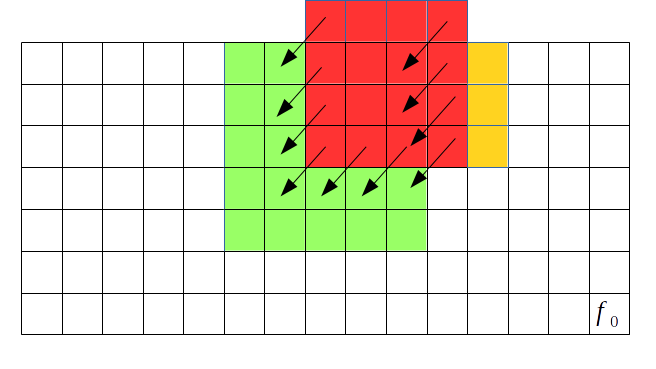
\includegraphics[width=0.7\linewidth]{../media/find-contours-spread-f0}
		\caption{Visualisierung von Ausbreiten und Wandern, erster Frame $f_0$. Die Vektoren geben die Bewegung des quadratischen Objekts an.}
		\label{fig:find-contours-spread-f0}
		\end{figure}
		\begin{figure}[H]
		\centering
		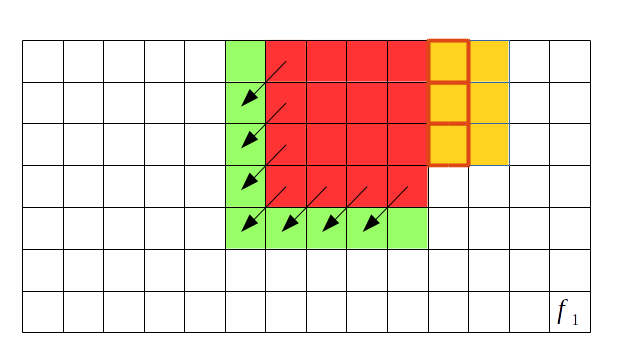
\includegraphics[width=0.7\linewidth]{../media/find-contours-spread-f1}
		\caption{Visualisierung des zweiten Frames $f_1$. Besonderes Augenmerk sollte auf das Weiterziehen der rechten Kante des roten Quadrats und dem damit verbundenen Farbwechsel der zuvor roten Pixel, verdeutlicht durch die orange Umrandung.}
		\label{fig:find-contours-spread-f1}
		\end{figure}


%		\subsection{Direkter Informationsgewinn aus Tiefenbildern}
					
		\subsection{Implementierung V1}
		
		\begin{itemize}
				\item Implementierung als ROS subscriber-node lauscht auf camera-depth-image topic von freenect\_launch
				\item OpenCV Fkt absdiff(absolute differential); braucht graustufe; benötigt 2 Bilder als eingabe liefert differenzielles Bild entweder in Bild1 zurück oder in übergebenen Ausgabespeicher
				\item ros eigene sensor-msgs images Nachrichten in OpenCV format bringen
%				\item wo liegt der Unterschied?
				\item in CMakelists.txt -> add\_executable + add\_library
				\item anpassungen bezüglich graustufenbilder in image\_converter.cpp
				\item Rauschen sehr instabil, Gauß Filter keinen Effekt
				\item Tiefenbilder zu Abhängig von Beleuchtung; schlecht
		\end{itemize}

		Unterschiede der beiden Bildcontainer:\\
		 \begin{itemize}
		 \item header | enthält diverse Infos über aktuellen Frame | std\_messages(kann int, String, double und weitere enthalten)
		 \item height | Höhe in Pixel | unit32 \\ 
		 \item width | Breite in Pixel | unit32\\
		 \item encoding | Bildkodierung RGB-24, mono8, mono13, ... | String\\ 
		 \item is\_bigendian | Orientierung des least significant bit | unit8\\
		 \item step | Zeilenlänge in Bytes relatiert Anzahl Spalten | unit32\\
		 \item data[] | Eigentlicher Bildinhalt als 2D-Array Spalten(step * Zeilenanzhal) | unit8\\
		 \end{itemize}
		 
		 \begin{itemize}
		 \item encoding | Bildkodierung RGB-24, mono8, mono13, ... | String\\ 
		 \item image[] | Eigentlicher Bildinhalt als 2D-Array Spalten(step * Zeilenanzhal) | MAT\\ 
		 \end{itemize}
		\textbf{(ADD)relevante Codeschnippsel in listing und erklären; Programmablaufplan zeichnen(ADD)}
						
		\subsection{Implementierung V2}
		\begin{itemize}
		\item rgb to mono weniger interferenz durch natürliches Licht; automatisch stabiler
		\item threshold sorgt für verteilung auf 2 Maxima, schwellwert-operation $I_p > \text{threshold} = \text{weiß}; I_p < \text{threshold} = \text{schwarz}$
		\item abprüfen ob Frame weiße Elemente enthält
		\item publish stop auf robotino-handler
		\end{itemize}
		\textbf{(ADD)PAP und Codeschnipsel(ADD)}			
		\section{Objekte Identifizieren}
		\begin{itemize}
		\item lediglich Unterscheidung ob Roboter oder Hindernis
		\item alles was nicht Roboter ist => Hindernis
		\item findobjekt ros
		\end{itemize}
			\subsection{Unterscheiden zwischen Roboter und Objekt}
			\begin{itemize}
			\item Robotino identifizieren -> Alleinstellungsmerkmal
			\item spezielles Muster? QR-Code? Abstraktes deutliches schwarz/weiß Design
			\item Skelett des Robotino anfertigen?
			\item Wie Perspektivische Unterschiede ausgleichen?
			\end{itemize}
		
	\chapter{Reaktion auf Hindernisse}
	\begin{itemize}
	\item bezug auf Klassifzierung
	\item Fallunterscheidung verdeutlichen
	\item Klassifikation anhand welcher Messwerte/Merkmale
	\end{itemize}
	\subsection{Klassifikation}
	\subsection{Bewegungsanalyse}
	\subsection{dynamische Objekte}
			\begin{itemize}
				\item Stop
				\item Bewegungsanalyse
				\item Hindernis kommt direkt auf Roboter zu -> weiterhin stehen bleiben
				\item Hindernis stoppt und bewegt sich nicht mehr weiter -> Umgehung bestimmen, umfahren
				\item Hindernis stoppt und bewegt sich weiter -> Roboter bleibt solange stehen bis Hindernis den Bewegungsraum verlassen hat oder sich nicht mehr weiter im Raum bewegt(stillstand) 
			\end{itemize}
	\subsection{statische Objekte}
	\subsection{chaotische Objkte}
	\subsection{Blitz Objekte}
